\documentclass[12pt]{article}
%\usepackage{algpseudocode} 
%\usepackage{algo}
\usepackage{fullpage,url,amssymb,epsfig,color,xspace,tikz,amsmath}
\usetikzlibrary{shapes,positioning,calc,chains}
\usepackage[pdftitle={CS 240 Assignment 3},%
pdfsubject={University of Waterloo, CS 240, Fall 2021},%
pdfauthor={MP}]{hyperref}
\RequirePackage{pstricks,pst-node,pst-tree} % draw trees, requires using xetex
\newlength{\nodeLength}
\newcommand{\Node}{A}
\newcommand{\setnode}[1]{
	\settowidth{\nodeLength}{#1}
	\renewcommand{\Node}[1]{
		\Tcircle[name=#1]{\makebox[\nodeLength]{##1}}
	}
}
\setnode{99}

% \snode{ID}{NUMBER} becomes \node{ID}[item]{\ensuremath{NUMBER}}
\newcommand{\snode}[2]{\node(#1)[item]{\ensuremath{#2}}}

% \nodelabel{SUBSCRIPT} becomes \node[label]{\ensuremath{S_SUBSCRIPT}}
\newcommand{\nodelabel}[1]{\node[label]{\ensuremath{S_#1}}}

\newcommand{\quesbox}[2]{\begin{center} \framebox[.5\textwidth]{%
			\raisebox{-5mm}[0mm][#1]{\begin{minipage}[t]{.45\textwidth}%
					{\normalsize\sf #2}{\phantom{ans}}\end{minipage}}} \end{center}}
\newcommand{\ceil}[1]{\left\lceil#1\right\rceil}
\newcommand{\floor}[1]{\left\lfloor#1\right\rfloor}
\renewcommand{\thesubsection}{Problem \arabic{subsection}}
\definecolor{typo}{rgb}{0.75,0,0}
\definecolor{care}{rgb}{0,0,0}
\begin{document}
	
	\begin{center}
		{\Large\bf University of Waterloo}\\
		\vspace{3mm}
		{\Large\bf CS240 Fall 2021}\\
		\vspace{2mm}
		{\Large\bf Assignment 3}\\
		\vspace{3mm}
		\textbf{Due Date: Wednesday, Nov 3 at 5:00pm}
	\end{center}
	
	\definecolor{care}{rgb}{0,0,0}
	\def\question#1{\item[\bf #1.]}
	\def\part#1{\item[\bf #1)]}
	\newcommand{\pc}[1]{\mbox{\textbf{#1}}} % pseudocode
	
	The integrity of the grade you receive in this course is very important to you and 
	the University of Waterloo.  As part of every assessment in this course you must read 
	and sign an Academic Integrity Declaration before you start working on the assessment and
	submit it \textbf{before the deadline of November 3rd} along with your answers to the 
	assignment; i.e. \textbf{read, sign and submit A03-AID.txt now or as soon as possible}.
	The agreement will indicate what you must do to ensure the integrity of your grade.
	If you are having difficulties with the assignment, course staff are there to help
	(provided it isn't last minute). \\
	~\\
	\textbf{The Academic Integrity Declaration must be signed and submitted on time or the
		assessment will not be marked.} \\
	~\\
	Please read
	\url{http://www.student.cs.uwaterloo.ca/~cs240/f20/guidelines.pdf} for guidelines on submission.  
	\textbf{Each question must be submitted individually to MarkUs as a PDF} with the corresponding file names: 
	a3q1.pdf, a3q2.pdf, ... , a3q6.pdf . \\
	~\\
	It is a good idea to submit questions as you go so you aren't trying to create several PDF files at the last minute. \\
	~\\
	\textbf{Late Policy:} Assignments are due at 5:00pm.
	To accommodate any small time differences with our submission server, there is a grace period of 5 minutes; i.e. we will accept assignments until 5:05pm without penalty.  Assignments submitted after 5:05pm will incur a penalty of 1 mark per minute to a maximum of 10 marks.   \\
	\textbf{Assignments submitted after 5:15pm will not be accepted}  
	but may be reviewed (by request) for feedback purposes only. \\  
	~\\
	
	
	%%%%%%%%%%%%%%%%%%%%%%%%%%%%%%%%%%%%%%%%%%%%%%%%%%%%%%%%%%%%%
	%%% Problem 1
	\subsection{[0+2+2=4 marks]}
	
	\begin{enumerate}
		\part{a} {\bf Practice} (not worth any marks):  Starting with an empty AVL tree, insert the following keys in order: 27 99 17 28 42 16 1 2 4. \\
		
		You should obtain the AVL tree given in the next part.
		
		\part{b} Given the following AVL tree: \\
		Note: this tree shows balance factors instead of height.
		
		\begin{center}
			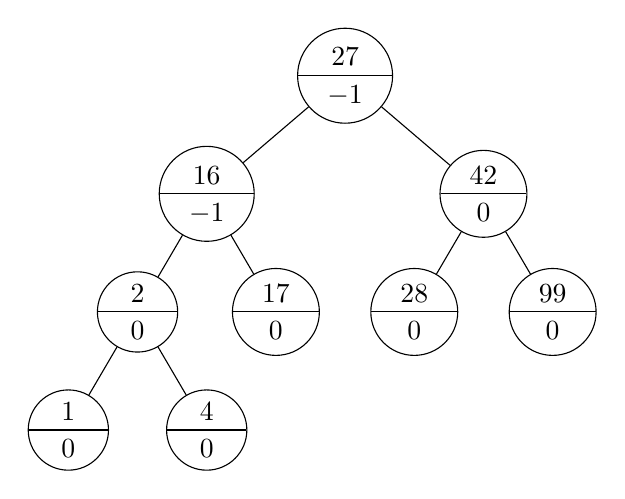
\begin{tikzpicture}[
				every node/.style = {draw, shape = circle split, grow = down},
				level 1/.style={sibling distance=100 pt},
				level 2/.style={sibling distance=50pt}]
				\node(z){$27$\nodepart{lower}$-1$}
				child{node{16\nodepart{lower}$-1$}
					child{node {2\nodepart{lower}$0$}
						child {node {1\nodepart{lower}$0$}}
						child {node {4\nodepart{lower}$0$}}}
					child{node {17\nodepart{lower}$0$}}
				}
				child{
					node{42\nodepart{lower}$0$}
					child{node {28\nodepart{lower}$0$}}
					child{node {99\nodepart{lower}$0$}}
				};
			\end{tikzpicture}
		\end{center}
		
		Insert the following keys in order:  8$^\star$, 22, 21, 18$^\star$.
		
		Show the resulting AVL trees with {\bf balance factors} (not height) for each node after the elements marked with star ($\star$) are inserted. \\
		Note: you should only show 2 trees.
		
		\part{c}  Consider the following AVL tree:
		\begin{center}
			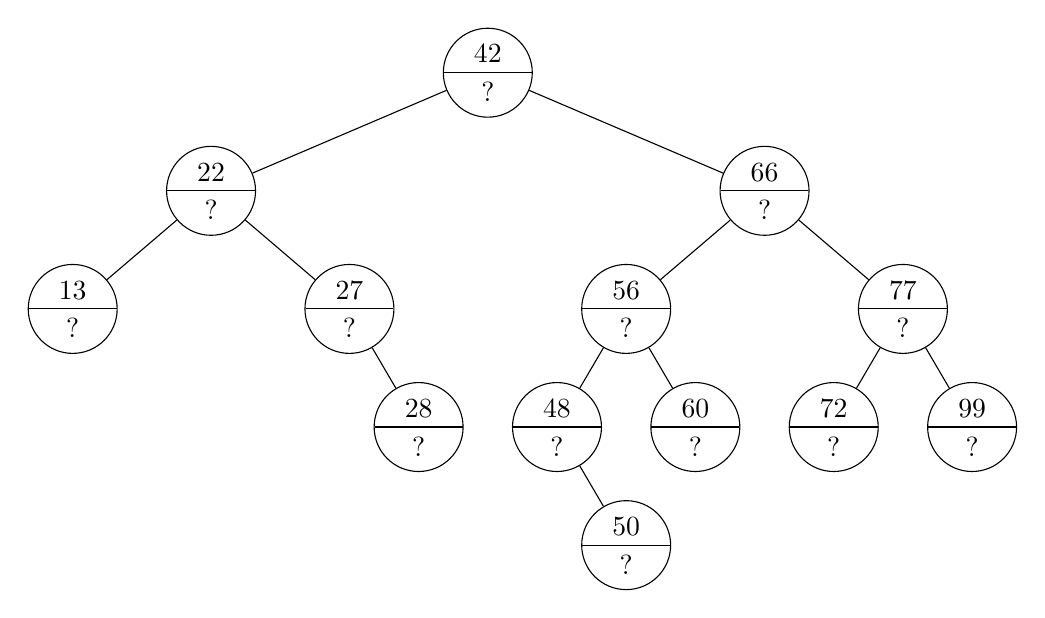
\begin{tikzpicture}[
				every node/.style = {draw, shape = circle split, grow = down},
				level 1/.style={sibling distance=200pt},
				level 2/.style={sibling distance=100pt},
				level 3/.style={sibling distance=50pt}]
				\node(z){$42$\nodepart{lower}$?$}
				child{node{22\nodepart{lower}$?$}
					child {node {13\nodepart{lower}$?$}}
					child {node {27\nodepart{lower}$?$}
						child[missing]
						child {node {28\nodepart{lower}$?$}}}}
				child {node {66\nodepart{lower}$?$}
					child {node {56\nodepart{lower}$?$}
						child {node {48\nodepart{lower}$?$}
							child[missing]
							child {node {50\nodepart{lower}$?$}}}
						child {node {60\nodepart{lower}$?$}}}
					child {node{77\nodepart{lower}$?$}
						child{node {72\nodepart{lower}$?$}}
						child{node {99\nodepart{lower}$?$}}}}
				;
			\end{tikzpicture}
		\end{center}
		
		Given the above tree, delete the following keys in order:
		
		\begin{center}
			66, 13$^\star$, 72, 77, 56$^\star$, 42$^\star$ 
		\end{center}
		
		Show the resulting AVL trees with {\bf balance factors} (not height) for each node after the elements marked with star ($\star$) are deleted.  
		If you have a choice of which element to move up, pick the inorder successor. \\
		Note: you should only show 3 trees.
		
	\end{enumerate}
	
	%%%%%%%%%%%%%%%%%%%%%%%%%%%%%%%%%%%%%%%%%%%%%%%%%%%%%%%%%%%%%
	%%% Problem 2
	\subsection{AVL Trees [4+6 marks]}
	
	In this question, we want to add support for an operation {\tt ithSuccessor} on AVL trees (in addition to the standard operations {\tt insert, delete, find}).
	The operation {\tt ithSuccessor} has two parameters, $x$ and $i \ge 0$, and returns the $i$th inorder successor of the node $x$.
	If $i = 0$, then the node $x$ itself is returned.
	You may assume that all input is valid; i.e. the successor exists (but may not be in the subtree rooted at $x$).
	
	We assume that the nodes have the following fields:
	\begin{itemize}
		\item {\tt key} -- the key of the node;
		\item {\tt left} -- pointer to the left child;
		\item {\tt right} -- pointer to the right child;
		\item {\tt balance} -- balance factor of the node;
		\item {\tt parent} -- pointer to the parent of the node;
		\item {\tt isLeft} -- is true if the node is a left child of its parent;
		\item {\tt isRight} -- is true if the node is a right child of its parent;
		\item {\tt numLeft} -- holds the number of nodes in the left subtree of the node;
		\item {\tt numRight} -- holds the number of nodes in the right subtree of the node.
	\end{itemize}
	
	\medskip
	
	\begin{enumerate}
		
		\part{a} Give an algorithm {\tt ithNode(x, i)} which returns the $i$th inorder node in the subtree rooted at $x$.
		For example, suppose the subtree contains $m$ nodes, when $i=1$, the minimum element in the subtree is returned and when $i=m$ the maximum element in the subtree is returned.
		You may assume that the subtree has at least $i$ elements.
		Your algorithm should take worst-case $O(\log(m))$ time.
		Briefly justify that your algorithm achieves this runtime.
		
		\part{b} Give the algorithm for {\tt ithSuccessor(x, i)} for an AVL tree with $n$ nodes.  
		Your algorithm should take worst-case $O(\log(n))$ time and must use {\tt ithNode(x, i)} from above.
		Briefly justify that your algorithm achieves this runtime.
	\end{enumerate}
	
	
	
	
	%%%%%%%%%%%%%%%%%%%%%%%%%%%%%%%%%%%%%%%%%%%%%%%%%%%%%%%%%%%%%
	%%% Problem 3
	\subsection{[3+3+4=10 marks]}
	
	Which of the following binary trees must have height $O(\log n)$?  Justify your answer.
	
	\begin{enumerate}
		\part{a} There is a constant $c > 0$ such that for all nodes $z$ in $T$, $z.left.height \leq z.right.height + c$.
		\part{b} Every node $z$ that is not a leaf in $T$ has exactly two children.
		\part{c} Given a BST $T$, let $N(z)$ be the number of nodes in the subtree rooted at $z$.
		If $z$ is an empty subtree, then $N(z) = 0$. \\
		There is a constant $0 < c \leq 1$ such that for every node $z$ in $T$, $N(z.left) \geq c\times N(z.right) - 1$ and $N(z.right) \geq c\times N(z.left) - 1$.
	\end{enumerate}
	
	%%%%%%%%%%%%%%%%%%%%%%%%%%%%%%%%%%%%%%%%%%%%%%%%%%%%%%%%%%%%%
	%%% Problem 4
	\subsection{[0+2+1+2+2+2=9 marks]}
	
	\begin{enumerate}
		\part{a} Practice (not worth any marks): Starting with an empty skip list, insert the following keys in order: 22 31 77 7 21 42 using the following flip sequence:
		
		\begin{center}
			HHTHTHHHTHHTHTHT
		\end{center}
		
		You should obtain the skip list given in the next part.
		
		\part{b} Given the following skip list:
		
		\begin{center}
			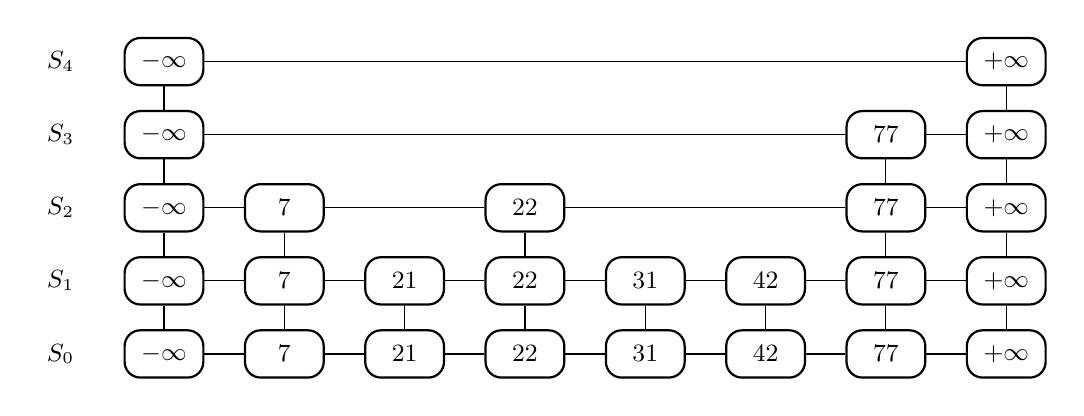
\begin{tikzpicture}[
				start chain,
				every node/.style={font=\small},
				item/.style={rectangle,minimum height=6mm,minimum width=10mm,
					rounded corners=2mm,thick,draw=black},
				label/.style={rectangle,minimum size=6mm}
				]
				
				% The nodes of the skip list are drawn in a matrix
				% \\ delimits the rows while & delimits the columns
				\matrix[row sep=3mm, column sep=5mm]{
					% Row 4: -infty ... +infty
					\nodelabel{4}; & \snode{4a}{-\infty}; & & & & & & & \snode{4n}{+\infty};\\
					
					% Row 3: -infty ... +infty
					\nodelabel{3}; & \snode{3a}{-\infty}; & & & & & & \snode{3l}{77}; & \snode{3n}{+\infty};\\
					
					% Row 2: -infty ...  ... +infty
					\nodelabel{2}; & \snode{2a}{-\infty}; & \snode{2c}{7}; & & \snode{2f}{22}; 
					& & & \snode{2l}{77}; & \snode{2n}{+\infty};\\
					
					% Row 1: -infty ...  ... +infty
					\nodelabel{1}; & \snode{1a}{-\infty}; & \snode{1c}{7}; & \snode{1e}{21}; & \snode{1f}{22}; 
					& \snode{1h}{31}; & \snode{1j}{42}; & \snode{1l}{77}; & \snode{1n}{+\infty};\\
					
					% Row 0: -infty 7 21 22 31 42 77 +infty
					\nodelabel{0}; & \snode{0a}{-\infty}; & \snode{0c}{7};  & \snode{0e}{21}; & \snode{0f}{22}; 
					& \snode{0h}{31};  & \snode{0j}{42};  & \snode{0l}{77};  & \snode{0n}{+\infty};\\
				};
				
				% Start chaining the nodes together
				{
					% Horizontal chains
					% Specify a starting node (by ID), and join to other nodes (by going "through" them in an unbroken line)
					% Eg row 2: Start at 2a, join 2e, join 2h, join 2i
					[start chain] \chainin(0a); \chainin(0c) [join]; \chainin(0e) [join]; \chainin(0f) [join]; \chainin(0h) [join];
					\chainin(0j) [join]; \chainin(0l) [join]; \chainin(0n) [join];
					[start chain] \chainin(1a); \chainin(1c) [join]; \chainin(1e) [join]; \chainin(1f) [join]; \chainin(1h) [join];
					\chainin(1j) [join]; \chainin(1l) [join]; \chainin(1n) [join];       
					[start chain] \chainin(2a); \chainin(2c) [join]; \chainin(2f) [join]; \chainin(2l) [join]; \chainin(2n) [join];
					[start chain] \chainin(3a); \chainin(3l) [join]; \chainin(3n) [join];
					[start chain] \chainin(4a); \chainin(4n) [join];
				}
				{
					% Vertical chains
					% Need to be separate chains from the horizontal ones
					[start chain] \chainin(0a); \chainin(1a) [join]; \chainin(2a) [join]; \chainin(3a) [join]; \chainin(4a) [join]; 
					[start chain] \chainin(0c); \chainin(1c) [join]; \chainin(2c) [join];
					[start chain] \chainin(0e); \chainin(1e) [join]; 
					[start chain] \chainin(0f); \chainin(1f) [join]; \chainin(2f) [join];
					[start chain] \chainin(0h); \chainin(1h) [join]; 
					[start chain] \chainin(0j); \chainin(1j) [join]; 
					[start chain] \chainin(0l); \chainin(1l) [join]; \chainin(2l) [join]; \chainin(3l) [join];
					[start chain] \chainin(0n); \chainin(1n) [join]; \chainin(2n) [join]; \chainin(3n) [join]; \chainin(4n) [join]; 
					
				}
			\end{tikzpicture}
		\end{center}
		
		
		Show the skip list that is created by inserting the keys: 37, 66, 13, 4, 27, 99 \\
		into the given skip list.  You must use the following coin flip sequence:
		\[
		HHHHTTHTHTHHTHTTHHHHHTHHTT
		\]
		Note that each coin flip in the sequence will only be used once, in order
		and there may be some unused coin flips.
		
		After inserting all keys, determine the exact number of comparisons (between 2 keys) required to search for the keys inserted in this part (that is, indicate what the search cost would be for 37, and then the search cost for 66, and so on).
		
		For example, a search for 18 in the given skip list above, requires 6 comparisons.
		
		\begin{center}
			\begin{tabular}{|c||c|c|c|c|c|c|} \hline
				Key &  37 &  66 &  13 &  4 & 27 & 99 \\ \hline
				Comparisons &   &   &   &   &  &  \\ \hline
			\end{tabular}
		\end{center}
		
		For the remaining parts, assume that the probability of adding a level to a tower is $p$ ($0 < p < 1)$, as opposed to $\frac{1}{2}$.
		
		\part{c} Explain why the probability that a key in the skip list has height at least $i$ is $p^i$.
		
		\part{d} Show that the expected number of extra nodes (i.e., the total number of nodes in skip list not including the nodes in $S_0$) is $O(n)$. 
		Therefore, the space requirements for this skip list are linear in the number of keys being stored.
		
		\part{e} Similar to what was done in lecture, let $C(k)$ be the expected total path length which rises $k$ levels when working back to the top-most, left-most node.  
		Find the recurrence relation for $C(k)$ in terms of $k$ and $p$. 
		
		\part{f} Assuming $C(0) = 0$, show that your recurrence relation from the previous part has closed form $C(k) = k/p$. 
		
	\end{enumerate}
	
	
	
	%%%%%%%%%%%%%%%%%%%%%%%%%%%%%%%%%%%%%%%%%%%%%%%%%%%%%%%%%%%%%
	%%% Problem 5
	\subsection{[2+2+2=6 marks]}
	
	Consider the list of keys:
	\[
	[1\ 2\ 3\ 4\ 5\ 6\ 7\ 8\ 9\ 10]
	\]
	and assume we perform the following searches:
	\begin{center}
		8, 6, 3, 7, 5$^\star$, 5, 2, 6, 2, 8$^\star$, 3, 9, 3, 8$^\star$ 
	\end{center}
	\begin{enumerate}
		\part{a} Using the move-to-front heuristic, give the list ordering after the starred ($\star$) searches are performed. 
		Additionally, record the number of comparisons between keys after each search, as well as, the total number of comparisons.
		\begin{center}
			\begin{tabular}{|c|c|c|c|c|c|c|c|c|c|c|c|c|c||c|} \hline
				8 &  6 &  3 &  7 &  5 & 5 & 2 & 6 & 2 & 8 & 3 & 9 & 3 & 8  & Total \\ \hline
				& & & & & & & & & & & & & & \\ \hline
			\end{tabular}
		\end{center}
		
		\part{b} Repeat part (a), using the transpose heuristic instead of the move-to-front heuristic.
		
		\part{c} Another heuristic is \textit{move-to-front2 (MTF2)} that is similar to
		\textit{move-to-front (MTF)} except that when an element is found at position $i$ it is moved to position $\left \lfloor \frac{i}{2} \right \rfloor$.  
		Repeat part (a), using this heuristic.  
		
	\end{enumerate}
	
	
	%%%%%%%%%%%%%%%%%%%%%%%%%%%%%%%%%%%%%%%%%%%%%%%%%%%%%%%%%%%%%
	%%% Problem 6
	\subsection{[2+2+2+2=8 marks]}
	
	\begin{enumerate}
		\part{a} Insert the following binary keys into an initially empty (uncompressed) binary trie:
		\begin{center}
			0110\$,\ 110\$,\ 0000\$,\ 01001\$,\ 01\$,\ 00\$,\ 01011\$,\ 0\$,\ 111\$,\ 010\$,\ 11\$
		\end{center}
		\part{b} From your answer to part (a), delete the following keys, and show the trie after each deletion:
		\begin{center}
			01011\$,\ 00\$,\ 0110\$ 
		\end{center}
		
		\part{c}  Repeat part (a), except use a compressed trie.
		
		\part{d}  Repeat part (b), starting from your answer to part (c).
	\end{enumerate}
	
	%%% END OF QUESTIONS %%%
\end{document}